% Author: Joshua Carey
% Description: Introduction chapter.
\let\textcircled=\pgftextcircled
\chapter{Introduction and Motivation}\label{chap:intro}

\initial{M}aritime travel has been a cornerstone of human civilisation, facilitating the exchange of goods, ideas, and cultures around the globe. The annals of history are full with instances of seafaring civilisation harnessing the power of wind to propel their vessels across the oceans. It is posited that ancient Neanderthals embarked on maritime voyages in the southern Ionian Islands between 110 to 35ka BP$~$\cite{Ferentinos2012}. The quintessence of maritime travel has predominantly been wind-powered sails, which remained unchallenged until the industrial revolution ushered in the era of fuel-powered engines.

The art and science of sailing have evolved significantly over millennia, from rudimentary rafts and canoes to sophisticated sailing ships with complex rigging systems. Ancient civilisation, including the Egyptians, Phoenicians, and Polynesians, made remarkable advancements in sailing technology, enabling them to explore and trade over larger swathes of the ocean$~$\cite{casson1995ships}. The medieval period saw the advent of the compass and the astrolabe, which further facilitated maritime navigation and exploration. The Age of Discovery, epitomised by the voyages of Columbus, Vasco da Gama, and Magellan, was propelled by advancements in sailing technology, which enabled transoceanic voyages and the establishment of maritime empires.

The industrial revolution in the 18th and 19th centuries marked a significant turning point in maritime propulsion. The invention of the steam engine heralded the decline of wind-powered sailing and the rise of fuel-powered propulsion systems. Steam-powered ships and later, diesel-powered ships, offered greater reliability, speed, and capacity compared to their wind-powered predecessors, thus becoming the preferred mode of maritime transportation$~$\cite{gardiner1993advent}. The transition to fuel-powered engines also mirrored the broader industrial and technological advancements of the era, which prioritised speed, efficiency and profit over traditional methods.

\section{A Renewed Interest in Wind Propulsion}
The environmental costs of fuel-powered maritime transportation have become increasingly apparent in the modern era. The shipping industry is a notable contributor to global carbon emissions, and the negative effects of pollution on marine ecosystems around the world are well-documented$~$\cite{corbett2007mortality}. These challenges have rekindled interest in wind propulsion as a sustainable alternative, prompting a re-examination of the principles that guided ancient and medieval sailors. The modern iteration of wind propulsion seeks to amalgamate the age-old wisdom of harnessing wind power with contemporary technological advancements to create eco-friendly and efficient maritime transportation systems.

Contemporary wind propulsion technologies like Flettner rotors$~$\cite{vahs2019retrofitting}, wing sails, and kite systems are being revisited to mitigate the environmental impact of maritime travel. Among these, kite-powered vessel technology stands out due to its potential for higher efficiency and ease of retrofitting. Kites offer two main advantages over traditional sails: they can move relative to the vessel, generating their own apparent wind and can be flown at higher altitudes, accessing different wind systems, where the wind is stronger and more consistent. The relative movement of a kite generates apparent wind, allowing for it to generate near its maximum potential force even when the vessel is stationary. This enhanced apparent wind results in a larger force compared to a sail of equivalent area.

However, the effective operation of kite-powered vessels requires precise control, which is skill-intensive. To leverage the full benefits of kites as a scalable propulsion method, implementing autonomous control is crucial. 

Reinforcement Learning (RL), a subset of machine learning, presents a compelling avenue for optimising the autonomous control of kite-powered vessels. RL, which is based on learning through interaction with an environment, offers a potential for developing advanced control systems and strategies that could greatly improve the effectiveness of kite-powered vessels. 


% The objective of this paper is to delineate a novel Reinforcement Learning approach aimed at optimising the autonomous control of kite-powered vessels. By leveraging the prowess of RL, we endeavor to address the challenges inherent in autonomous sail control, thereby contributing to the overarching goal of sustainable and efficient maritime transportation. The ensuing discourse will elucidate the theoretical underpinnings of our approach, the experimental setup, and the empirical findings, underscoring the potential benefits in terms of reducing operational costs and mitigating environmental impact.


% \section{Project Definition}

% How can reinforcement Learning techniques be effectively applied to autonomously control a kite-powered vessel?

% This project aims to develope a simulation environment that can be used to train an RL agent to autonomously control a kite-powered vessel. The development of a simulation environment is crucial, attempting to train an agent to fly a kite let alone navigate a boat in the real world would not be feasible; the simulation environment will allow for the agent to learn in a safe and controlled fashion, not to mention the iteration time and cost will be significantly reduced. However simulation creates its own issues. Integration into the real world becomes an significant factor, how realistic is good enough? What features of the real world are the most important to implement? How do we know if the agent will be able to perform in the real world? These are all questions that will be considered throughout the project. 

% The kite-powered vessel in question is displayed in figure XYZ, and is comprised of a boat hull and LEI (leading edge inflatable) kite, connected by 4 control lines, this configuration is further explained in section$~$\ref{sec:env}. 

% Autonomous control is a broad term, in this case it means enabling self-governance of the vessel control functions with no human input. For the purpose of this project the agent will be trained to navigate the kiteboat towards a target location (waypoint). The better the agent performs this task, the harder the problem will become with waypoints moving to different locations. This process if taken to its extreme could represent full autonomous control, with the entire navigation and control down to the agent. `Control', what does control mean in this scenario. The agent will have a number of actions, these will represent steering the boats rudder and flying the kite. A single agent will be trained to control both the kite and the boat, this makes the learning problem more complicated but was attempted as a novel approach to create a system that had full control of the vessel. In this vein success is two-fold, the agent must be able to fly the kite reliably while continuously steering towards the next waypoint.

% For any machine learning endeavor, especially one with such intricate physical dynamics, the choice of simulation environment is paramount. Not only does it provide the playground for our AI agent to learn and make mistakes safely, but it also serves as a litmus test for the robustness and realism of the designed model.

% Given the myriad of choices available, the Unity game engine emerged as the most suitable platform. Its native support for machine learning applications through the MLAgents toolkit was unmatched. Beyond its reputation in gaming, the inherent support for mesh bodies, colliders, and a variety of joints made it an attractive option for simulating the kite-boat system, which comprised a complex dance of forces, and counterforces. Unity is recognised for its potent physics engine, however for this project the use of Unity's physics engine will be kept to a minimum, with an emphasis on implementing as much of the simulation from scratch as possible. Unity will be used primarily for its visual capabilities and the ability to be used as the gym environment for machine learning simulations. 

% Central to this simulation is the depiction of water, the medium in which the boat will navigate. Here, the Unity HDRP Water System 16.0.3$~$\cite{UnityHDRPWaterSystem}, bundled with Unity 2023.2.0b9, provides a realistic representation of water with its undulating waves, refractions, and reflections. 

% The alternative option to using Unity's water system was to model an entire particle fluid simulation, this would have had its advantages, however it would have been a lot more computationally expensive and would have taken a lot longer to implement. As this project was primarily focused on training a RL algorithm for controlling a kiteboat it was decided that the Unity water system would be sufficient for this project.  

\section{Project Definition}

\subsection{Research Question}
How can reinforcement learning (RL) techniques be effectively applied to autonomously control a kite-powered vessel?

\subsection{Objective and Scope}
This project focuses on developing a simulation environment to train an RL agent for autonomous control of a kite-powered vessel. Given the impracticality of directly training in the real world due to safety concerns, cost, and time constraints, the simulation environment offers a controlled and cost-effective alternative. However, this approach raises critical questions about realism and integration with real-world conditions: What level of realism is sufficient? Which real-world features are crucial to simulate? How can we ensure the agent's real-world performance?

\subsection{Vessel Configuration}
% The kite-powered vessel, detailed in figure$~$\ref{kiteboat_diagram}, consists of a boat hull and a Leading Edge Inflatable (LEI) kite, connected by four control lines. The configuration and mechanics of this setup are elaborated in section$~$\ref{sec:env}.

The kite-powered vessel that will be used in this project is based on the concept of taking an existing recreational boat and attaching a mass produced Leading Edge Inflatable (LEI) kite to it. Figure$~$\ref{kiteboat} shows a Silent 60$~$\cite{silent} electric catamaran with a Core$~$\cite{core} LEI kite attached to the front with the Wingit Kite Control system, which is discussed in section$~$\ref{sec:kiteboat_tech}. Figure$~$\ref{fig:kiteboat} shows the kiteboat model that was created for this project, this model is based on a monohull boat with a LEI kite attached to the front. The configuration and mechanics of this setup are elaborated in section$~$\ref{sec:env}. 

% minipage with two images side by side
\begin{figure}[!htb]
    \centering
    \begin{minipage}[t]{0.45\textwidth}
        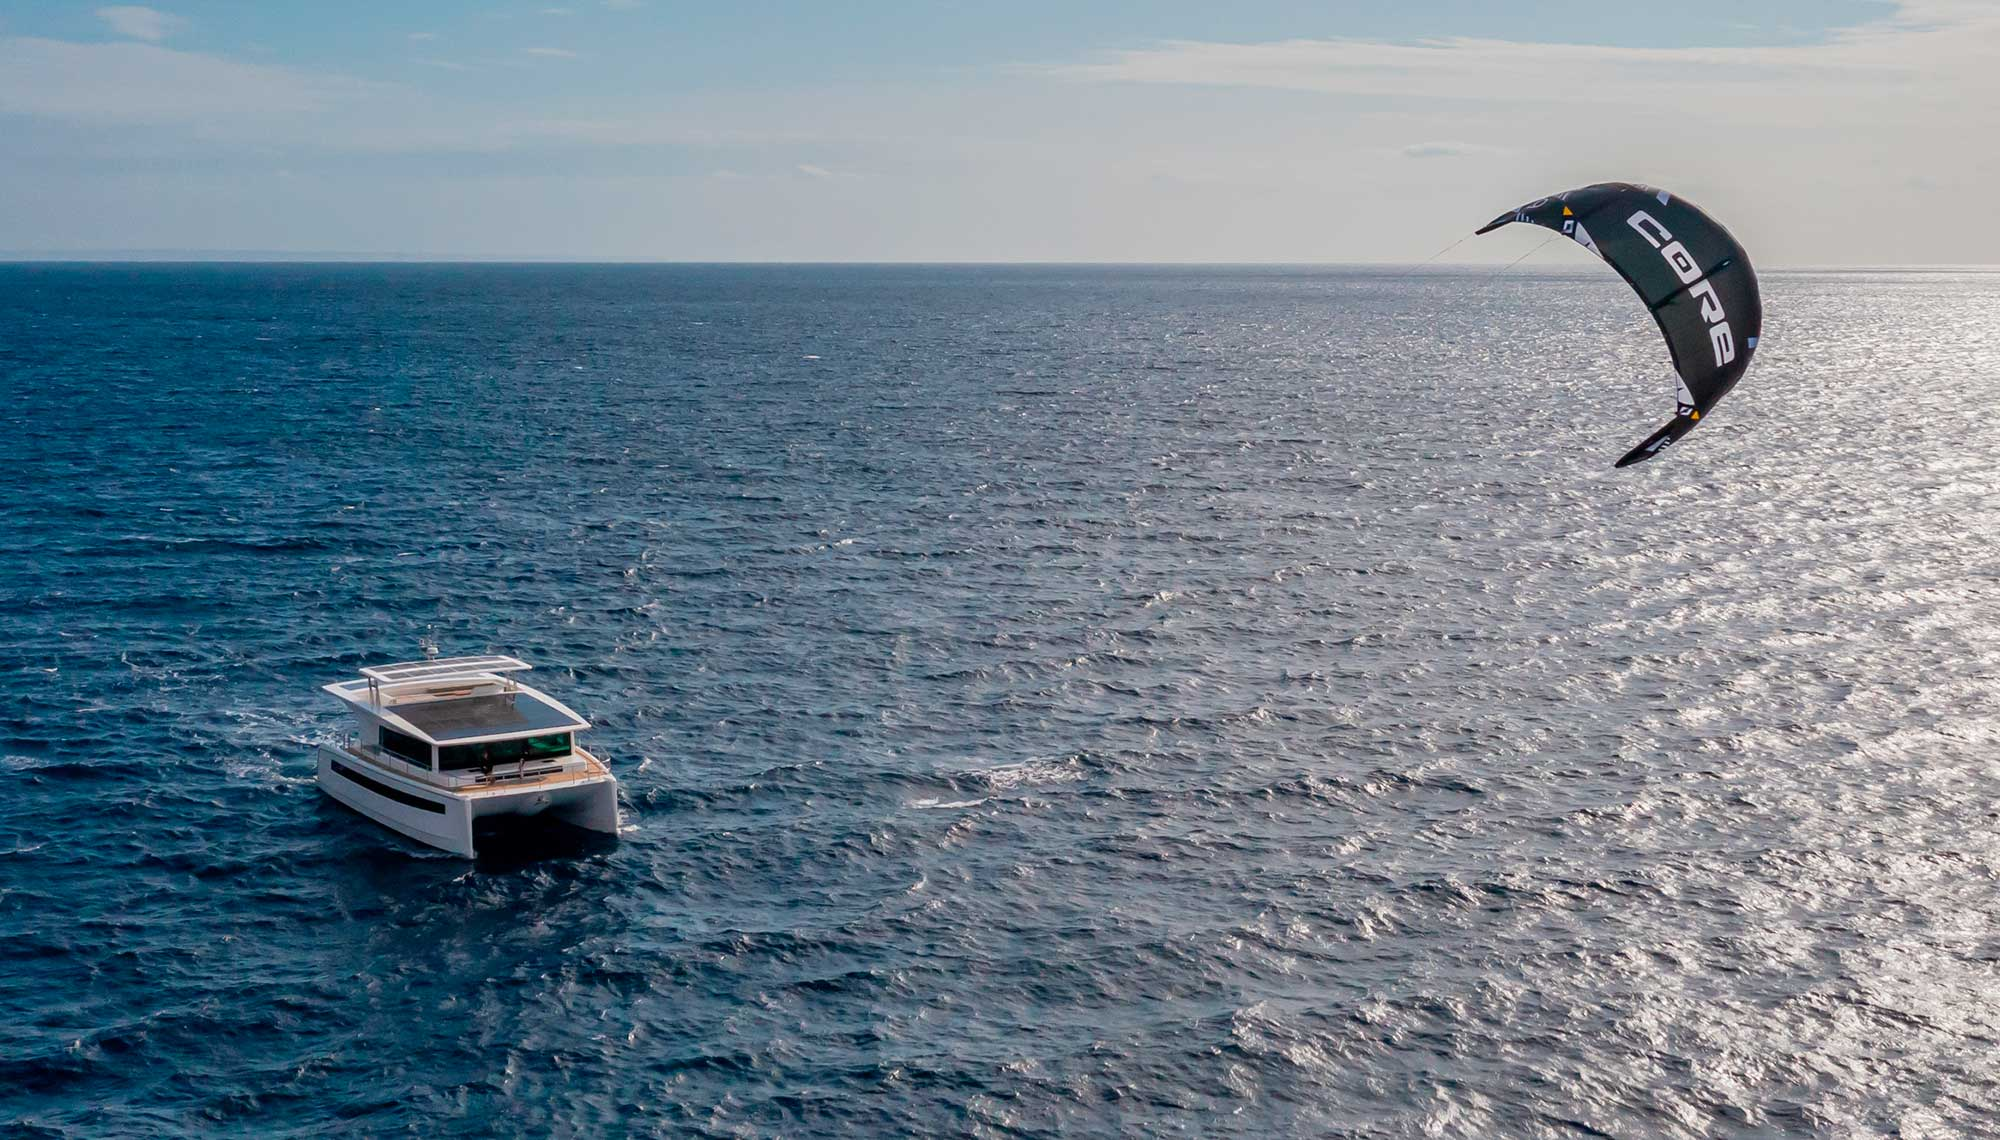
\includegraphics[width=\linewidth]{Images/kiteboat.jpg}
        \caption{Silent 60 with Wingit Kite Control}\label{kiteboat}
    \end{minipage}\hfill
    \begin{minipage}[t]{0.45\textwidth}
        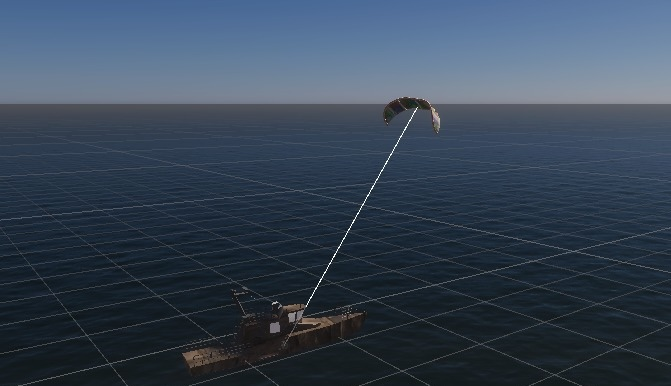
\includegraphics[width=\linewidth]{Images/kiteboat_diagram.png}
        \caption{Simulation Kiteboat}\label{fig:kiteboat}
    \end{minipage}
\end{figure}


\subsection{Autonomous Control Definition}
In this context, 'autonomous control' refers to enabling the vessel to operate independently without human intervention. The primary training objective for the RL agent is to navigate the kiteboat towards varying waypoints, increasing in difficulty as the agent's performance improves. This escalating challenge aims to approximate full autonomous navigation and control. 'Control' in this scenario encompasses steering the boat's rudder and managing the kite's flight. A single agent is tasked with managing both aspects, presenting a complex but novel challenge in achieving comprehensive vessel control.

\subsection{Simulation Environment}
The choice of the simulation environment is crucial, given the complex physical dynamics involved in machine learning. Unity game engine, with its MLAgents toolkit, was selected for its exceptional support for machine learning applications, realistic physics engine, and robust visual capabilities. Unity serves primarily as the visual interface and the 'gym' for machine learning simulations.

\subsection{Simulation Components}
Central to this simulation is the representation of water, a key element in the boat's navigation. Unity HDRP Water System 16.0.3 (Unity 2023.2.0b9) offers a realistic depiction of water dynamics, essential for the project's fidelity. While a complete particle fluid simulation was considered, it was deemed excessively computationally intensive and time-consuming for the project's primary focus—training the RL algorithm for kiteboat control. Therefore, Unity's water system was chosen for its balance of realism and efficiency.


% \subsection{Impact and Real-World Application}

% The implications of successfully applying reinforcement learning to autonomously control a kite-powered vessel extend far beyond the academic sphere. This project holds significant potential for real-world applications, particularly in maritime industries and autonomous navigation technologies.

% \textbf{Sustainable Marine Navigation}: Kite-powered vessels offer an eco-friendly alternative to traditional maritime transportation, relying on wind power to reduce fuel consumption and carbon emissions. By achieving autonomous control, these vessels can become more viable for commercial use, contributing to greener maritime operations.

% \textbf{Autonomous Transportation}: This research contributes to the broader field of autonomous vehicle technologies. The insights gained from controlling a complex system like a kiteboat can inform the development of autonomous systems in other domains, such as aerial drones or self-driving cars.


\section{Aims and Objectives}

The overarching aim of this research is to develope a system for controlling kite-powered vessels using Reinforcement Learning (RL) techniques. This objective stems from the need to advance sustainable maritime travel technologies and reduce the environmental impact of current propulsion systems. 

To achieve this primary aim, the objectives have been structured as follows:

\subsection*{Objective 1: Simulation Environment Development}
\begin{itemize}
    \item To design and implement a virtual marine environment that accurately emulates real-world maritime conditions.
    \item To construct a realistic model of a boat that exhibits appropriate physical movements in response to environmental forces such as wind and water currents.
    \newline\textbf{Outcome Goal:} To have a physics-based boat able to be controlled and driven around a scene by a human player.
\end{itemize}

\subsection*{Objective 2: Kite Propulsion Modeling}
\begin{itemize}
    \item To create a physics-based model of a kite within the simulation that reflects authentic aerodynamic behaviours and integrate it onto the boat model.
    \item To integrate kite control mechanics into an agent’s available action space.
    \newline\textbf{Outcome Goal:} To have a physics-based kiteboat able to be controlled and driven around a scene by a human player, using an agent's heuristic controls.
\end{itemize}

\subsection*{Objective 3: Reinforcement Learning Framework Establishment}
\begin{itemize}
    \item To formulate a set of observations, actions, and rewards that encapsulate the dynamics of autonomous kite-boat control and navigation.
    \item To deploy the Proximal Policy Optimisation algorithm, leveraging its actor-critic method for effective policy learning.
    \newline\textbf{Outcome Goal:} To have an agent begin training using PPO to learn to control the kiteboat.
\end{itemize}

\subsection*{Objective 4: Autonomous Agent Development}
\begin{itemize}
    \item To develop an RL agent capable of learning basic control and manoeuvres, starting with simple navigating towards a target and maintaining a constant course.
    \item To refine the agent's capability to adaptively control the kite's position and angle to optimise propulsion for speed while navigating towards a target.
    \newline\textbf{Outcome Goal 1:} To have an agent that can navigate towards a target in a straight line.
    \newline\textbf{Outcome Goal 2:} To have an agent that can navigate towards a target in any direction, including using manoeuvres to take the optimal path.
\end{itemize}

\subsection*{Objective 5: Efficacy and Optimisation Testing}
\begin{itemize}
    \item To utalise High-Performance Computing (HPC)$~$\cite{HPC} resources for scaling up simulations and optimising the training process.
    \item To rigorously evaluate the trained agent’s performance in simulating autonomous navigation in various environmental scenarios.
    \newline\textbf{Outcome Goal 1:} To train an agent using the HPC resources.
    \newline\textbf{Outcome Goal 2:} To have an agent that can navigate towards a target in a straight line under various environmental conditions, including wind and waves.
\end{itemize}

\subsection*{Objective 6: Real-World Applicability Assessment}
\begin{itemize}
    \item To extrapolate simulation findings to assess real-world applicability and propose a  practical deployment of RL in kite-powered vessels.
    \item To provide recommendations for further research and development based on empirical results obtained from the simulation studies.
\end{itemize}

These objectives pave the path towards achieving the central goal, ensuring each phase of development builds upon the last. By concluding this research it is anticipated that the contributions made could impact sustainable maritime transportation solutions.



% @article{Ferentinos2012,
%     author = {Ferentinos, G. and Gkioni, M. and Geraga, M. and Papatheodorou, G.},
%     title = {Early seafaring activity in the southern Ionian Islands, Mediterranean Sea},
%     journal = {Journal of Archaeological Science},
%     volume = {39},
%     number = {7},
%     pages = {2167-2176},
%     year = {2012},
%     doi = {10.1016/J.JAS.2012.01.032},
%     url = {https://dx.doi.org/10.1016/J.JAS.2012.01.032}
% }
% @book{Balard2017,
%     editor = {Balard, Michel and Buchet, Christian},
%     title = {The Sea in History - The Medieval World},
%     publisher = {Boydell \& Brewer, Boydell Press},
%     year = {2017},
%     edition = {NED - New edition},
%     pages = {1086},
%     url = {https://www.jstor.org/stable/10.7722/j.ctt1kgqt6m}
% }